%%%%%%%%%%%%%%%%%%%%%%%%%%%%%%%%%%%%%%%%%%%%%%%%%%%%%%%%%%%%%%%%%%%%%%%%%%%%%%%
%%
%%          $Id: Rulebook.tex 2014-12-12 balkce $
%%    author(s): RoboCupAtHome Technical Committee(s)
%%  description: introduction to RoboCupAtHome
%%
%%%%%%%%%%%%%%%%%%%%%%%%%%%%%%%%%%%%%%%%%%%%%%%%%%%%%%%%%%%%%%%%%%%%%%%%%%%%%%%
\documentclass[11pt, twoside, openright, a4paper, chapterprefix]{scrbook}
\usepackage[inner=2.5cm, outer=2.5cm, top=4cm, bottom=4cm]{geometry}

%%% PACKAGES %%%%%%%%%%%%%%%%%%%%%%%%%%%%%%%%%%%%%%%%%%%%%%%%%%%%%%%%%%%%%%%%%%
%%%%%%%%%%%%%%%%%%%%%%%%%%%%%%%%%%%%%%%%%%%%%%%%%%%%%%%%%%%%%%%%%%%%%%%%%%%%%%%
%%
%%          $Id: packages.tex 385 2013-02-12 21:53:10Z holz $
%%    author(s): RoboCupAtHome Technical Committee(s)
%%  description: List of packages for the RoboCupAtHome rulebook
%%
%%%%%%%%%%%%%%%%%%%%%%%%%%%%%%%%%%%%%%%%%%%%%%%%%%%%%%%%%%%%%%%%%%%%%%%%%%%%%%%
\usepackage{soul}

\usepackage[english]{babel}
\usepackage{amsmath,amssymb,amsfonts}
\usepackage[nice]{nicefrac}
\usepackage{siunitx}
\usepackage{graphicx}
\usepackage{multicol}
\usepackage{fancyhdr}
\usepackage{svn-multi}
\usepackage{color}
\usepackage{xcolor,colortbl}
\usepackage{epsfig}
\usepackage{makeidx}
\usepackage{lscape}
\usepackage{picinpar}
% \usepackage{./styles/bar}
\usepackage{./styles/tweaklist}
%\usepackage{subfigure}
\usepackage{enumerate,paralist}
\usepackage{multirow}
\usepackage{pgffor}
\usepackage{array}
\usepackage{etoolbox}
\usepackage{hyperref}
\usepackage{tabularx}
\usepackage{xspace}

%\usepackage[utf8x]{inputenc}
%\usepackage{times}
%\usepackage{helvet}
%\usepackage{courier}

\usepackage{url}
\usepackage{caption}
%\usepackage{subcaption}
\usepackage{epstopdf}
\usepackage{subfig}
\usepackage{float}
\usepackage{wrapfig}
\usepackage{titlesec}
\usepackage{xfrac}

% Local Variables:
% TeX-master: "../../rulebook"
% End:


%%% SubfigureSetup %%%%%%%%%%%%%%%%%%%%%%%%%%%%%%%%%%%%%%%%%%%%%%%%%%%%%%%%%%%%
%\renewcommand{\subfigtopskip}{5pt}        % default is 10pt
%\renewcommand{\subfigbottomskip}{5pt}     % default is 10pt
%\renewcommand{\subfigcapskip}{3pt}        % default is 10pt
%\renewcommand{\subfigcapmargin}{7pt}      % default is 10pt

%%% TweakList-Setup %%%%%%%%%%%%%%%%%%%%%%%%%%%%%%%%%%%%%%%%%%%%%%%%%%%%%%%%%%%
\renewcommand{\itemhook}{%                 % modify itemize-spacing
  \setlength{\topsep}{2pt}%
  \setlength{\partopsep}{1pt}%
  \setlength{\itemsep}{-1pt}%
}
\renewcommand{\enumhook}{%                 % modify enumerate-spacing
  \setlength{\topsep}{2pt}%
  \setlength{\partopsep}{1pt}%
  \setlength{\itemsep}{-1pt}%
}
\renewcommand{\descripthook}{%             % modify description-spacing
  \setlength{\topsep}{2pt}%
  \setlength{\partopsep}{1pt}%
  \setlength{\itemsep}{-1pt}%
}

\setkomafont{title}{\normalfont}
\setkomafont{sectioning}{\normalfont\bfseries}
\addtokomafont{caption}{\small}
\setkomafont{captionlabel}{\small\bfseries}
\setkomafont{descriptionlabel}{\normalfont\bfseries}
\renewcommand*{\chapterformat}{\LARGE{Chapter \thechapter}}

%%% MACROS %%%%%%%%%%%%%%%%%%%%%%%%%%%%%%%%%%%%%%%%%%%%%%%%%%%%%%%%%%%%%%%%%%%%
% \newcommand{\YEAR}{2012}
% \newcommand{\STATE}{Final}

\newcommand{\YEAR}{2015}
\newcommand{\STATE}{Draft}
\graphicspath{{\YEAR/}{./general/images/}}
%%%%%%%%%%%%%%%%%%%%%%%%%%%%%%%%%%%%%%%%%%%%%%%%%%%%%%%%%%%%%%%%%%%%%%%%%%%%%%%
%%
%%          $Id: macros.tex 399 2013-02-14 20:24:02Z holz $
%%    author(s): RoboCupAtHome Technical Committee(s)
%%  description: Macros for the RoboCupAtHome rulebook
%%
%%%%%%%%%%%%%%%%%%%%%%%%%%%%%%%%%%%%%%%%%%%%%%%%%%%%%%%%%%%%%%%%%%%%%%%%%%%%%%%

%%%%%%%%%%%%%%%%%%%%%%%%%%%%%%%%%%%%%%%%%%%%%%%%%%%%%%%%%%%%%%%%%%%% 
% Macros for generating score sheets for RoboCup@Home              %
% to be used in the rulebook or during the competition             %
%                                                                  % 
% Author: Dirk Holz & David Gossow                                 %
% Modif : Mauricio Matamoros                                       %
% $Id: macros_score_sheets.tex 429 2013-04-30 10:09:55Z holz $     %
%%%%%%%%%%%%%%%%%%%%%%%%%%%%%%%%%%%%%%%%%%%%%%%%%%%%%%%%%%%%%%%%%%%% 


\usepackage{calc}
\usepackage{ifthen}
\usepackage{wasysym}
\usepackage{chngpage}


%%% Counters / temp. variables %%%%%%%%%%%%%%%%%

\newcounter{currTestScore}
\newcounter{currTestScoreTotal}
\newcounter{currTestScoreTotalWithoutBonus}
\newcounter{currOutstandingBonus}
\newcommand{\scorelistOptions}{}
\newcommand{\scoresheetOptions}{}

% set \shortScoresheet to true for the rulebook version and to false for the referee's scoresheet
\newcommand{\shortScoresheet}{true}

% set \threeAttempts to true for three columns in the scoresheet
\newcommand{\threeAttempts}{false}

% set \retryAvailable to true for a second column in the scoresheet
\newcommand{\retryAvailable}{true}

% set \continueAvailable to true for CONTINUE sections
\newcommand{\continueAvailable}{true}

% set \dataRecordingBonus to true for data recording bonus
\newcommand{\dataRecordingBonus}{true}

% name of the current test, is set automatically in the rulebook
\newcommand{\currentTest}{}

% (internal) if-clause shortcut to switch between short rulebook version and full score sheet for referees
\newcommand{\ifShortScoresheet}[2]{%
  \ifthenelse{ \equal{\shortScoresheet}{true}}{%
    #1%
  }{%
    #2%
  }%
}

\newcommand{\ifEvaluationSheet}[2]{%
  \ifthenelse{ \equal{\scoresheetOptions}{evaluationSheet}}{%
    #1%
  }{%
    #2%
  }%
}

% (internal) draws the scoresheet line for score handwritting
\newcommand{\scoreline}[1][0.08]{\rule{#1\linewidth}{.2pt}}

% (internal) draws the lines for score hadndwritting in the table outline based on the number of attempts
\newcommand{\attemptScoreLines}{
  \switchAttempts
    {\scoreline[0.06] & \scoreline[0.06] & \scoreline[0.06]}
    {\scoreline & \scoreline}
    {\scoreline}
}

% (internal) Select one of the provided arguments based on the number of attempts
% (3 tries, retry (2) or only try (1))
\newcommand{\switchAttempts}[3]{
  \ifthenelse{\equal{\threeAttempts}{true}}{#1}{\ifthenelse{\equal{\retryAvailable}{true}}{#2}{#3}}
}

% (internal) stores the number of attempts to perform
\edef\numAttempts{0}
% (internal) writes on the command \numAttempts the number of attempts to perform
\newcommand\defNumAttempts{
  \switchAttempts
  {\global\edef\numAttempts{3}}
  {\global\edef\numAttempts{2}}
  {\global\edef\numAttempts{1}}
}

%% commands for overriding internal calculations %%%%%%%%%%%%%%%%%%%%%%%%%%%%%%%%%%%%%%%%

% set score counter to arbitrary value
\newcommand{\setTotalScore}[1]%
{%
  \setcounter{currTestScore}{#1}
}

% set outstanding bonus to arbitrary value
\newcommand{\setOutstandingBonus}[1]%
{%
  \setcounter{currOutstandingBonus}{#1}
}




%% Score sheet page layout %%%%%%%%%%%%%%%%%%%%%%%%%%%%%%%%%%%%%%%%%%%%%%%%%%%%%%%%%%%%%%%%

% usage: \begin{scoresheet}[repeatable] ... \end{scoresheet}
\newenvironment{scoresheet}[1][]{
  % begin
  \newpage

  \renewcommand{\scoresheetOptions}{#1}
  
  \begin{minipage}[t]{0.8\textwidth}%
    \vspace{0pt}
    {\huge \textbf{Score Sheet} }
    
    \vspace{2 em}
    
    \begin{tabular}{ @{} l l l}
      \textbf{Test:} & \currentTest \\[.9 em]
      
      \ifEvaluationSheet{}{%
        \textbf{Team name:} & \scoreline[0.6]\\[.9 em]%
      }%
      % 
      \textbf{Referee name:} & \scoreline[0.6]\\[.9 em]%
      %	
      %	\ifEvaluationSheet{}{%
      %   \textbf{Restart:} & \Square ~1st try \hspace{1 em} \Square ~2nd try
      %	}
      %	
      % test repetition checkboxes (for stage 2 tests)
      \ifthenelse{ \equal{#1}{repeatable} }{%
	\textbf{Test repetition:} & \Square ~1st \hspace{1 em} \Square ~2nd\\[.9em]%
      }{}
    \end{tabular}

    \vspace{0.5 em}

  \end{minipage}
  \hfill
  \begin{minipage}[t]{0.15\textwidth}%
    \vspace{0pt}
    
\includegraphics[width=\textwidth]{images/logo_RoboCupAtHome.jpg}%
  \end{minipage}\\
}
{
  % end
  \vspace{.2 em}
  \textbf{Remarks:}

  %% signatures of referee / team leader %%%%%%%%%%%%
  \vfill
  \ifEvaluationSheet{
    % team evaluation sheet
    \begin{tabular}{@{} @{\extracolsep{\fill}} l l @{}}
      \scoreline[0.25] \hspace{0.05\linewidth} & \scoreline[0.25] \hspace{0.05\linewidth}
      \\
      \textit{Date \& time}%
      & \textit{Referee}
    \end{tabular}
  }{
    % normal sheet
    \begin{tabular}{@{} @{\extracolsep{\fill}} l l l @{}}
      \scoreline[0.25] \hspace{0.05\linewidth} & \scoreline[0.25] \hspace{0.05\linewidth} & \scoreline[0.25]
      \\
      \textit{Date \& time}%
      & \textit{Referee} %
      & \textit{Team leader}
    \end{tabular}
  }

  \newpage
}


%% Score list table %%%%%%%%%%%%%%%%%%%%%%%%%%%%%%%%%%%%%%%%%%%%%%%%%%%%%%%%%%%%%%%%

% usage: \begin{scorelist}[openDoorSignal] ... \end{scorelist}
\newenvironment{scorelist}[1][]{
  % begin

  % init variables %%%%%%%%%
  \renewcommand{\scorelistOptions}{#1}
  \setcounter{currTestScore}{0}
  \setcounter{currOutstandingBonus}{0}

  % setup table %%%%%%%%%
  \vspace{0.8 em}

  \ifShortScoresheet {
    \begin{tabular*}{\textwidth}{@{} @{\extracolsep{\fill}} p{0.8\linewidth} r @{}}
      \ifEvaluationSheet{
        \textbf{Team} & \textbf{Score} \\ \hline 
      }{%
        \textbf{Action} & \textbf{Score} \\ \hline 
      }
    }{  
      % else:
      % \begin{tabular*}{\textwidth}{@{}p{0.65\linewidth}lp{0.15\linewidth}@{}}
      %   \textbf{Action} & \textbf{Score} & \multicolumn{1}{l}{\textbf{Success}}\\ \hline 
      \ifEvaluationSheet{
        \begin{tabular*}{\textwidth}{@{} @{\extracolsep{\fill}} p{0.7\linewidth} r r @{}}
          \textbf{Team} & \textbf{Score} & \textbf{Result}\\ \hline 
        }{
          \ifthenelse{\equal{\threeAttempts}{true}}{
            \begin{tabular*}{\textwidth}{@{} @{\extracolsep{\fill}} p{0.6\linewidth} r r r r @{}}
            \textbf{Action} & \textbf{Score} & \textbf{\small $1^{st}$ try} & \textbf{\small $2^{nd}$ try} & \textbf{\small$3^{rd}$ try} \\ \hline 
          }
          %else
          {
            \begin{tabular*}{\textwidth}{@{} @{\extracolsep{\fill}} p{0.6\linewidth} r r r @{}}
            \textbf{Action} & \textbf{Score} \ifthenelse{\equal{\retryAvailable}{true}}{& \textbf{1st try} & \textbf{2nd try}}{ & \textbf{Only try}} \\ \hline 
          }
        }
      }
    }
      {
        % end

	\ifEvaluationSheet{}{%
          
          % calculate max. score, outstanding bonus %%%%%%%
          \ifthenelse{\value{currOutstandingBonus} = 0}{%
            \setcounter{currOutstandingBonus}{ \value{currTestScore} / 10 }
          }{}
          \setcounter{currTestScoreTotal}{ \value{currTestScore} + \value{currOutstandingBonus} }
          \setcounter{currTestScoreTotalWithoutBonus}{ \value{currTestScore} }
          

          % Special penalties & bonuses %%%%%%%%%%%%%%%%
          \scoreheading{Special penalties \& standard bonuses}

          \ifthenelse {\equal{\dataRecordingBonus}{true}}{\scoreitem{10}{Contributing with recorded data ($\frac{\sum gathered\ points}{max\ points} \times$) \ifShortScoresheet{(see sec.~\ref{rule:datarecording})}{}}}{}
          
          \scoreitem{-50}{Not attending \ifShortScoresheet{(see sec.~\ref{rule:not_attending})}{}}
          
          \ifthenelse{\equal{\scorelistOptions}{openDoorSignal}}{
            \scoreitem{-10}{Using start button \ifShortScoresheet{(see sec.~\ref{rule:start_button})}{}}
          }{}

          % \ifthenelse{\value{currOutstandingBonus} = 0}{
          \scoreitem{\thecurrOutstandingBonus}{Outstanding performance \ifShortScoresheet{(see sec.~\ref{rule:outstanding_performance})}{}}
          % }{}
          
          % Total score %%%%%%%%%%%%%%%%
          \hline\\
          % \textbf{Total score} & \scoring{ \thecurrTestScoreTotal } %
          \ifShortScoresheet {%
            % No Score per try in short version
          }{%
            \textbf{\textit{Score per try}} & \scoring{ \thecurrTestScoreTotalWithoutBonus } %
          }
          % add line to put in total:
          \ifShortScoresheet{}{& \attemptScoreLines} \\   
          \ifShortScoresheet{
            \textbf{Total score} (excluding penalties and bonuses) & \scoring{ \thecurrTestScoreTotalWithoutBonus } %
          }{
            \defNumAttempts
            & \\
            \textbf{Total score}  & \scoring{ \thecurrTestScoreTotalWithoutBonus } & \multicolumn{\numAttempts}{c}{\scoreline[0.20]}
          } \\
	}

      \end{tabular*}
      
    }


    %% Score sheet table entries %%%%%%%%%%%%%%%%%%%%%%%%%%%%%%%%%%%%%%%%%%%%%%%%%%%%%%%%%%%%%%%%

    % for loop helper
    % usage: \forloop[step]{counter}{initial_value}{conditional}{code_block} 
    \newcommand{\forloop}[5][1]%
    {%
      \setcounter{#2}{#3}%
      \ifthenelse{#4}%
      {%
 	#5%
 	\addtocounter{#2}{#1}%
 	\forloop[#1]{#2}{\value{#2}}{#4}{#5}%
      }%
      % else
      {%
      }%
    }

    \newcounter{ct}

    % heading
    % usage: \scoreheading{text}
    \newcommand{\scoreheading}[1]{
      \ifShortScoresheet {%
        \phantom{.} \\[-4 ex] \multicolumn{2}{@{}l}{\textbf{\textit{#1}}}\\[0pt]
      }{%
        \phantom{.} \\[-4 ex] \multicolumn{3}{@{}l}{\textbf{\textit{#1}}}\\[0pt]
      }
    }

    % table entry
    % usage: \scoreitem[multiplicity]{points}{description}
    \newcommand{\scoreitem}[3][1]{

      % add to max. total score if points > 0
      \ifthenelse{ #2 > 0 }{
        \addtocounter{currTestScore}{ #2 * #1 }
      }{}%
      % 
      \begin{minipage}[t]{\linewidth} {#3} \vspace{0.1 em} \end{minipage} & %
      \scoring{ \ifthenelse{ \equal{#1}{1} }{}{ #1 $\times$} \ifthenelse{ \equal{#2}{0} }{}{ #2}}%
      % insert check marks:	
      %	\ifShortScoresheet{}{ & \forloop{ct}{0}{\value{ct} < #1}{ \Square}} \\[3pt]
      % insert line
      \ifShortScoresheet{ %
        \\ 
      }{ % else
        \ifEvaluationSheet{}{& \attemptScoreLines} \\[0pt]
      }
    }


% Local Variables:
% TeX-master: "../Rulebook"
% End:

%%%%%%%%%%%%%%%%%%%%%%%%%%%%%%%%%%%%%%%%%%%%%%%%%%%%%%%%%%%%%%%%%%%%%%%%%%%%%%%
%%
%%          $Id: macros_open_demonstrations.tex 391 2013-02-14 07:57:07Z sugiura $
%%    author(s): holz
%%  description: simple macros for specifications of open challenges
%%
%%%%%%%%%%%%%%%%%%%%%%%%%%%%%%%%%%%%%%%%%%%%%%%%%%%%%%%%%%%%%%%%%%%%%%%%%%%%%%%

\newcommand{\OpenDemonstrationTask}[2] {
  \begin{enumerate}%
    \item \textbf{Setup and demonstration:} The team has a maximum of \timing{#1 minutes} for setup, presentation and demonstration.%
    \item \textbf{Interview and cleanup:} After the demonstration, there is
	      another \timing{#2 minutes} where the team answers %
    questions by the jury members.\\%
    During the interview time, the team has to undo its changes to the environment.%
  \end{enumerate}%
}

\newcommand{\OpenDemonstrationChanges}{
  \subsection{Changes to the environment}
  \begin{enumerate}
    \item \textbf{Making changes:} As in the other open demonstrations, teams are allowed to make modifications to the arena as they like, 
    but under the condition that they are reversible.
    \item \textbf{Undoing changes:} In the interview and cleanup team, changes need to be made undone by the team. 
    The team has to leave the arena in the \emph{very same} condition they entered it.
  \end{enumerate}
}
% Local Variables:
% TeX-master: "../Rulebook"
% End:


\newcommand{\rulebookVersion}{\STATE\ version for RoboCup \YEAR\xspace(\VERSION)}

\def\RoboCup{{\textsc{RoboCup}}}
\def\Robocup{{\textsc{RoboCup}}}
\def\robocup{{\textsc{RoboCup}}}
\def\AtHome{{\textsc{RoboCup@Home}}}
\def\MSL{\textsc{Middle Size League}}
\def\MS{{\textsc{Middle Size}}}
\def\SSL{\textsc{Soccer Simulation League}}
\def\SS{\textsc{Soccer Simulation}}

\def\TC{technical committee (TC)}
\def\OC{organizing committee (OC)}

\renewcommand{\labelenumi}{\arabic{enumi}.}
\renewcommand{\labelenumii}{\labelenumi\arabic{enumii}.}
\renewcommand{\labelenumiii}{\labelenumii.\arabic{enumiii}.}


%% %%%%%%%%%%%%%%%%%%%%%%%%%%%%%%%%%%%%%%%%%%%%%%%%%%%%%%%%% %%
%%                    Developement-Tools                     %%
%% %%%%%%%%%%%%%%%%%%%%%%%%%%%%%%%%%%%%%%%%%%%%%%%%%%%%%%%%% %%

%% %%%%%%%%%%%%%%%%%%%%%%%%%%%%%%%%%%%%%%%
\newcommand{\tbc}[1]{\textbf{\it\color{red}{t.b.c. ...}#1\color{black}}}
\newcommand{\todo}[1]{\textbf{\it\color{red}{todo: }#1\color{black}}}
\newcommand{\TODO}[1]{\textbf{\it\color{red}{TODO:\\}#1\color{black}}}
\newcommand{\chk}[1]{\textbf{\color{red}#1\color{black}}}

\newcommand{\reworkon}{\marginpar{\raggedright\color{red}{$\downarrow$rework}\color{black}}}
\newcommand{\reworkoff}{\marginpar{\raggedright\color{red}{$\uparrow$rework}\color{black}}}

%% %%%%%%%%%%%%%%%%%%%%%%%%%%%%%%%%%%%%%%%
%%  site notes/margin notes
\def\note#1{\marginpar{\raggedright\tiny#1}}
\def\mpar#1{\marginpar{\raggedright\tiny#1}}
\def\rand#1{\marginpar{\raggedright\tiny#1}}
\setlength{\marginparwidth}{2cm}

\newcommand{\refsec}[1]{Section~\ref{#1}}
\newcommand{\reftab}[1]{Table~\ref{#1}}
\newcommand{\reffig}[1]{Figure~\ref{#1}}

%% %%%%%%%%%%%%%%%%%%%%%%%%%%%%%%%%%%%%%%%
%% side-annotation-macros for easy lookup
% \newcommand{\awardmark}{\marginpar{\centering
\includegraphics[width=.34cm]{images/icon_award.pdf}}}
% \newcommand{\refmark}{\marginpar{\centering
\includegraphics[width=.5cm]{images/icon_whistle.pdf}}}
% \newcommand{\referee}[1]{\emph{#1}\marginpar{\centering
\includegraphics[width=.5cm]{images/icon_whistle.pdf}}}
% \newcommand{\scoremark}{\marginpar{\centering
\includegraphics[width=.34cm]{images/icon_score.pdf}}}
\newcommand{\awardmark}{}
\newcommand{\refmark}{}
\newcommand{\referee}[1]{}
\newcommand{\scoremark}{}
%\newcommand{\scoring}[1]{\emph{#1}\marginpar{\centering
\includegraphics[width=.34cm]{images/icon_score.pdf}}}
\newcommand{\scoring}[1]{\emph{#1}}
\newcommand{\timark}{\marginpar{\centering
\includegraphics[width=.34cm]{icon_clock.pdf}}}

%\newcommand{\timing}[1]{\emph{#1}\marginpar{\centering
\includegraphics[width=.34cm]{images/icon_clock.pdf}}}
\newcommand{\timing}[1]{\emph{#1}}

\def\revnumtmpfile{.temp_ruleook_version}
\def\revdattmpfile{.temp_ruleook_date}
\def\svnRevision{Unknown} %
\def\svnChangeData{Unknown} %
\immediate\write18{svnversion . > \revnumtmpfile}
\IfFileExists{\revnumtmpfile}{\def\svnRevision{\input{\revnumtmpfile}\unskip}}{} 
\immediate\write18{svn info | grep 'Last Changed Date:' | awk '{print $4}'> \revdattmpfile}
\IfFileExists{\revdattmpfile}{\def\svnChangeData{\input{\revdattmpfile}\unskip}}{} 
\newcommand{\VERSION}{Revision \svnRevision, \svnChangeData}
% \IfFileExists{\revnumtmpfile}{\immediate\write18{rm -f \revnumtmpfile}}{} 
% \IfFileExists{\revdattmpfile}{\immediate\write18{rm -f \revdattmpfile}}{} 
% Local Variables:
% TeX-master: "../../rulebook"
% End:

%% %%%%%%%%%%%%%%%%%%%%%%%%%%%%%%%%%%%%%%%%%%%%%%%%%%%%%%%%%%%%%%%%%%%%%%%%%%%
%%
%%          $Id: abbrevix.tex 373 2013-02-12 20:32:49Z holz $
%%    author(s): RoboCupAtHome Technical Committee(s)
%%  description: Abbreviations for the RoboCupAtHome RuleBook
%%
%% %%%%%%%%%%%%%%%%%%%%%%%%%%%%%%%%%%%%%%%%%%%%%%%%%%%%%%%%%%%%%%%%%%%%%%%%%%%

%% temp-variables %%%%%%%%%
\newlength{\adxtemp}
\newlength{\adxspace}
\setlength{\adxspace}{3cm}

%% %%%%%%%%%%%%%%%%%%%%%%%%%%%%%%%%%%%%%%%
%%  Commands to use this
%% %%%%%%%%%%%%%%%%%%%%%%%%%%%%%%%%%%%%%%%

%% \abb{abk}
%% to reference an abbreviation
\newcommand{\abb}[1]{\hypertarget{#1}{#1}}

%% \term{the term}
%% print 'the term' in italic,
%% do not include 'the term' in index
%\newcommand{\term}[1]{#1\index{#1}}
\newcommand{\term}[1]{\textit{#1}}

%% \iterm{the term}
%% print 'the term' in italic,
%% include 'the term' in index
\newcommand{\iterm}[1]{\textit{#1}\index{#1}}

%% \nterm{the term}
%% do NOT print 'the term' but include 'the term' in index
\newcommand{\nterm}[1]{\index{#1}}

%% \TERM
%% print first term, add second term to index
\newcommand{\Term}[2]{\textit{#1}\index{#2}}


%% \aterm{the term}{abb}
%% print 'term', 
%% include 'term' with abbreviation 'abb' in abbreviation-index
\newcommand{\aterm}[2]{\settowidth{\adxtemp}{#2}{\hypertarget{#2}{#1 (#2)}\abbex{#2\hspace{\adxspace}\hspace{-\the\adxtemp}#1}}}

%% \iaterm{the term}{abbreviation} 
%% print 'term', 
%% include 'the term' in index, 
%% and include abbreviation in abbreviation-index
\newcommand{\iaterm}[2]{\settowidth{\adxtemp}{#2}{\hypertarget{#1}{\textit{#1} (#2)}\index{#1}\abbex{#2\hspace{\adxspace}\hspace{-\the\adxtemp}#1}}}

%% %%%%%%%%%%%%%%%%%%%%%%%%%%%%%%%%%%%%%%%
%%  Main Abbreviation Definitions
%% %%%%%%%%%%%%%%%%%%%%%%%%%%%%%%%%%%%%%%%

\makeatletter
\newlength{\QZ@TOChdent}% Used to define hanging indents.
\setlength{\QZ@TOChdent}{1.0em}%
\renewcommand{\@pnumwidth}{1.55em}%
\makeatother
%
%\newenvironment{simpleenv}[4]{\clearpage}{\clearpage}%
%\newenvironment{simpleenv}[4]{\clearpage}{\pagebreak}%
\newenvironment{simpleenv}[4]{\pagebreak}{\pagebreak}%
\newcommand{\BaseDiff}{0}%
%\newcommand{\RSpnum}[1]{\makebox[\@pnumwidth][r]{#1}}%
\newcommand{\RSpnum}[1]{\makebox[1.57em][r]{#1}}%
\newcommand{\RSnopnum}[1]{\makebox[\@pnumwidth][r]{}}%
\newcommand{\RSpset}[1]{\RSpnum{#1}}%
%
\newcommand{\printabbex}[4][\jobname]{%
  \typeout{ ***** printabbex #1 #2 #3 #4 for file \jobname.tex}%
  \IfFileExists{#1.and}{%
     \begin{simpleenv}{#1}{#2}{#3}{#4}%
       \pagestyle{plain} %
       \addcontentsline{toc}{chapter}{#2}%
       \chapter*{\textbf{#3}}{#4}%
       \input{#1.and}%
       \vfill%
     \end{simpleenv}%
   }%
   {\typeout{ ***** ERROR: No file #1.and found for file \jobname.tex.}}}%
\renewcommand{\see}[2]{#2 \emph{see} #1}%
\makeatletter
\newcommand{\makeabbex}[1][\jobname]{\begingroup
  \makeatletter
  \if@filesw \expandafter\newwrite\csname #1@adxfile\endcsname
  \expandafter\immediate\openout \csname #1@adxfile\endcsname #1.adx\relax
  \typeout{ ***** Writing abbex file #1.adx for file \jobname.tex.}%
  \fi \endgroup}
%\makeatother
%\makeatletter
\@onlypreamble{\makeindex}%
\newcommand{\abbex}[2][\jobname]{\@bsphack\begingroup
               \def\protect##1{\string##1\space}\@sanitize
               \@wrabbex{#1}{#2}}
\newcommand{\@wrabbex}[2]{\let\thepage\relax
   \xdef\@gtempa{\@ifundefined{#1@adxfile}{}{\expandafter
      \write\csname #1@adxfile\endcsname{\string
      \indexentry{#2|}{\thepage}}}}\endgroup\@gtempa
   \if@nobreak \ifvmode\nobreak\fi\fi\@esphack}
\makeatother
\newcommand{\indxspace}{\par\vspace{\BaseDiff\baselineskip}}
\makeatletter
\newcommand{\IndexSet}{%
\renewcommand{\@idxitem}{\par\setlength{\leftskip}{0pt}%
                         \setlength{\hangindent}{\QZ@TOChdent}}%
\renewcommand{\subitem}{\par\setlength{\leftskip}{0.25in}%
                         \setlength{\hangindent}{\QZ@TOChdent}}%
\renewcommand{\subsubitem}{\par\setlength{\leftskip}{0.5in}%
                         \setlength{\hangindent}{\QZ@TOChdent}}%
\renewcommand{\indexspace}{}
\renewcommand{\indxspace}{\par\vspace{\BaseDiff\baselineskip}}
\renewenvironment{theindex}{%
                \setlength{\parindent}{\z@}%
                \parskip\z@ \@plus .3\p@\relax
                \setlength{\rightskip}{\@tocrmarg}%
                \setlength{\parfillskip}{-\rightskip}%
                \let\item\@idxitem}
} %% End of the IndexSet definition
\makeatother

\newcommand{\printidx}{\addcontentsline{toc}{chapter}{Index}\printindex}
\newcommand{\printabx}{\printabbex{Abbreviations}{Abbreviations}{}}
%\newcommand{\printabbrevidx}{\printindex[abb]{Abk�rzungen}{Abk�rzungen}{}}
\newcommand{\printabbrevidx}{\printabbex{Abbreviations}{Abbreviations}{}}
%\newcommand{\makeabbrevidx}{\makeindex[abb]}
\newcommand{\makeabbrevidx}{\makeabbex}

% Local Variables:
% TeX-master: "../Rulebook"
% End:




\makeindex                                % generate index
\makeabbex                                % generate abbreviations

%%% DOCUMENTINFO %%%%%%%%%%%%%%%%%%%%%%%%%%%%%%%%%%%%%%%%%%%%%%%%%%%%%%%%%%%%%%
\hypersetup{
  pdftitle     = {RoboCup@Home Rules and Regulations},
  pdfsubject   = {RoboCup@Home Rulebook},
  pdfauthor    = {RoboCup@Home Technical Committee},
  pdfkeywords  = {RoboCup, @Home, Rules, Competition},
  colorlinks   = true,
  anchorcolor  = blue,
  linkcolor    = blue,
  urlcolor     = blue, 
}

%%% HEADINGS & PAGE STYLE %%%%%%%%%%%%%%%%%%%%%%%%%%%%%%%%%%%%%%%%%%%%%%%%%%%%%
\newcommand{\footline}{RoboCup@Home Rulebook / \rulebookVersion}
\pagestyle{fancy}
\renewcommand{\chaptermark}[1]{\markboth{\chaptername\ \thechapter. \ #1}{}}
\renewcommand{\sectionmark}[1]{\markright{\thesection \ #1}{}\renewcommand{\currentTest}{#1}}
\fancyhf{}
\fancyhead[LE,RO]{\thepage}
\fancyhead[RE]{\sffamily\rightmark}
\fancyhead[LO]{\sffamily\leftmark}
\fancyfoot[C]{\scriptsize \sffamily \footline{}}
\fancypagestyle{plain}{
        \fancyhf{}
        \fancyhead[LE,RO]{\thepage}
        \fancyhead[RE]{\sffamily\rightmark}
        \fancyhead[LO]{\sffamily\leftmark}
        \fancyfoot[C]{\scriptsize \sffamily \footline{}}
		\renewcommand{\headrulewidth}{0.5 pt}
}
\fancypagestyle{empty}{
        \fancyhf{}
        \fancyhead{}
        \fancyfoot[C]{\scriptsize \sffamily \footline{}}
		\renewcommand{\headrulewidth}{0 pt}
}

\newcommand{\quotes}[1]{``#1''}
\newcommand{\textbi}[1]{\textbf{\textit{#1}}}
%\newcommand{\sectionbreak}{\clearpage}
%\newcommand{\subsectionbreak}{\clearpage}


%%%%%%%%%%%%%%%%%%%%%%%%%%%%%%%%%%%%%%%%%%%%%%%%%%%%%%%%%%%%%%%%%%%%%%%%%%%%%%%
%%%%%%%%%%%%%%%%%%%%%%%%%%%%%%%%%%%%%%%%%%%%%%%%%%%%%%%%%%%%%%%%%%%%%%%%%%%%%%%
%%%%%%%%%%%%%%%%%%%%%%%%%%%%%%%%%%%%%%%%%%%%%%%%%%%%%%%%%%%%%%%%%%%%%%%%%%%%%%%

\begin{document}

%% %%%%%%%%%%%%%%%%%%%%%%%%%%%%%%%%%%%%%%%%%%%%%%%%%%%%%%%%%%%%%%%%%%%%%%%%%%%
%%
%%          $Id: titlepage.tex 428 2013-04-30 10:01:14Z holz $
%%    author(s): RoboCupAtHome Technical Committee(s)
%%  description: Title page for the RoboCupAtHome RuleBook
%%
%% %%%%%%%%%%%%%%%%%%%%%%%%%%%%%%%%%%%%%%%%%%%%%%%%%%%%%%%%%%%%%%%%%%%%%%%%%%%
\begin{titlepage}
  \begin{center}
    {
      
\includegraphics[width=.25\textwidth]{images/logo_RoboCupFed.jpg}
      \hfill
      
\includegraphics[width=.25\textwidth]{images/logo_RoboCupAtHome.jpg}\\[1.23ex]
    }
    \vspace{2.7 cm}
    \hrulefill\par
    {%
      \vspace*{.27cm}
      \Huge{RoboCup@Home}\\[1.23ex]
      \Large Rules \& Regulations \\[2ex]
    }
    \hrulefill\par
    \vfill
    ~~ Version: \YEAR \quad \svnRevision ~~ \\
    ~~ Last Build Date: \today \quad Time: \the\time ~~ \\
    ~~ \svnChangeData ~~ %\\
    %\vfill
  \end{center}
\end{titlepage}
% Local Variables:
% TeX-master: "../../rulebook"
% End:


\pagestyle{empty}
%% %%%%%%%%%%%%%%%%%%%%%%%%%%%%%%%%%%%%%%%%%%%%%%%%%%%%%%%%%%%%%%%%%%%%%%%%%%%
%%
%%          $Id: acknowledgments.tex 404 2013-02-15 08:51:20Z sugiura $
%%    author(s): RoboCupAtHome Technical Committee(s)
%%  description: Acknowledgments for the RoboCupAtHome RuleBook
%%
%% %%%%%%%%%%%%%%%%%%%%%%%%%%%%%%%%%%%%%%%%%%%%%%%%%%%%%%%%%%%%%%%%%%%%%%%%%%%



\section*{About this rulebook}
This is the official rulebook of the RoboCup@Home competition 2015.
It has been written by the 2014/2015 RoboCup@Home Technical Committee (in alphabetical order): 
Loy van Beek, 
Kai Chen, 
Dirk Holz,  
Mauricio Matamoros, 
Caleb Rascon, 
Maja Rudinac, 
Javier Ruiz des Solar, 
Komei Sugiura, and 
Sven Wachsmuth.

\section*{How to cite this rulebook}
If you refer to RoboCup@Home and this rulebook in particular, please cite:

Loy van Beek, Kai Chen, Dirk Holz, Mauricio Matamoros, Caleb Rascon, Maja Rudinac, Javier Ruiz des Solar, Komei Sugiura, and Sven Wachsmuth. 
``Robocup@Home 2015: Rule and regulations,'' 
\url{http://www.robocupathome.org/rules/2015_rulebook.pdf}, 2015.

\begin{verbatim}
@misc{ rulebook_2015,
  author =       {Loy van Beek AND Kai Chen AND Dirk Holz AND
  					Mauricio Matamoros AND Caleb Rascon AND
  					Maja Rudinac AND Javier Ruiz des Solar AND
  					Komei Sugiura AND Sven Wachsmuth},
  title =        {RoboCup@Home 2015: Rule and Regulations},
  year =         2015,
  howpublished = {\url{http://www.robocupathome.org/rules/2015_rulebook.pdf}},
}
\end{verbatim}

\section*{Acknowledgments}
\label{sec:acknowledgments}


We would like to thank all the people who contributed to the RoboCup@Home league 
with their feedback and comments. 
We also like to thank the members of the technical committee who put up the rules
and the organizing committee who organizes the competition.  

~\\\noindent People that have been working on this rulebook as member of one of the league's 
committees (in alphabetical order):
\begin{multicols}{2}%
\noindent%
Loy van Beek\\
Jean-Daniel Dessimoz\\
Peter Ford Dominey\\
Mohan Rajesh Elara\\
David Gossow\\
Dirk Holz\\
Luca Iocchi\\
Gerhard Kraetzschmar\\
Fariborz Mahmoudi\\
Mauricio Matamoros\\
Daniele Nardi\\
Sven Olufs\\
Caleb Rascon\\
Maja Rudinac\\
Javier Ruiz-del-Solar\\
Paul E. Rybski\\
Jesus Savage\\
Stefan Schiffer\\
J\"org St\"uckler\\
Komei Sugiura\\
Tijn van der Zant\\
Sven Wachsmuth\\
Thomas Wisspeintner\\ 
Jiongkun Xie\\
Amin Yazdani
\end{multicols}
% Local Variables:
% TeX-master: "../../rulebook"
% End:

\clearpage

\pagestyle{empty}
\tableofcontents
\clearpage

\pagestyle{plain}

\chapter{Introduction}
\todo{Write Introduction section}
\chapter{Concepts behind the competition}
\todo{Write Competition Concepts section}
\chapter{General rules \& Regulations}
\todo{Write General section}
\chapter{Setup and preparation}
\todo{Write Setup section}

\chapter{Tests in Stage I}

\begin{itshape}
All ability and integration tests in Stage I grants 15 points and are performed 3 times. The total score for each of this tests is the average of the best two performances (still to be discussed, perhaps taking only the top 1 or --unlikely-- global average).

Open/Demo Challenge and RoboZoo are special cases. Those tests grant up to 10 points each, and have no changes from previous years. In case of Open/Demo Challenge (most likely is going to be a focused Demo Challenge), scoring will be redefined.
\end{itshape}

\section{General Purpose Service Robot}

This test evaluates Human-Robot Interaction and the integration of the abilities of the robot tested in stage I. In this test the robot has to solve multiple tasks upon request. That is, the test is not incorporated into a (predefined) story and there is neither a predefined order of tasks nor a predefined set of actions. The actions that are to be carried out by the robot are randomly generated by the referees and are composed by 3 subtasks which include navigation, human-robot interaction and robot-object interaction.

The command is composed by three actions, which the robot has to show it has recognized. The robot may repeat the understood command and ask for confirmation. If it can't recognize the command correctly, it can also ask the speaker to repeat the complete command, or ask for further information.

\subsection{Focus}
This test particularly focuses on the following aspects:
\begin{itemize}
	\item No predefined order of actions to carry out (to get away from state machine-like behavior programming).
	\item Increased complexity in speech recognition (possible commands are less restricted in both actions/operators and arguments/objects, commands can include multiple objects, e.g., \quotes{put the apple on the kitchen table})
\end{itemize}

\subsection{Task}

\begin{enumerate}
	\item \textbf{Entering and command retrieval:} The robot enters the arena and drives to a designated position where it has to wait for further commands.
	\item \textbf{Command generation:} A command is generated randomly, depending on the command category chosen by the team (see below). \\

	\item \textbf{Command categories:} All possible actions has been classified previously by the TC according to their difficulty level. The team may choose from the following three categories:
	\begin{enumerate}
		\item \textbf{Category I:} Tasks with a low degree of difficulty (easy to solve). This category includes indoor navigation, grasping known objects, answering questions (from the predefined set of questions), etc.
		\item \textbf{Category II:} Tasks with a moderate degree of difficulty. This category includes following a human, indoor navigation in crowded environments, grasping alike objects, find a calling person (waving or shouting), etc.
		\item \textbf{Category III:} The same tasks as in category II. However, the information given to the robot will be incomplete or incorrect, meaning that the command as it is specified exactly is not possible. The robot must come up with an appropriate solution to meet the operators' command. Please see the Command examples below.
	\end{enumerate}

	\item \textbf{Task assignment:} The robot is given the command by the operator and may directly start to work on the task assignment. The robot must must prove it has understood the given command by repeating it (Please see the remarks about this in section~\ref{sec:gpsr_remarks}).
	\item \textbf{Exiting the arena:} After accomplishing the assigned task, the robot has to leave the arena.
\end{enumerate}

\subsection{Commands and actions}
The command is composed by three actions, which the robot has to show it has recognized. The robot may repeat the understood command and ask for confirmation. If it can't recognize the command correctly, it can also ask the speaker to repeat the complete command. If the robot fails to understand the given commands, it may ask to the operator to repeat them up to three times, if it fails the team may opt to use the Continue rule (Section \refsec{rule:asrcontinue}). In case the robot has understood partially the command, it may ask the operator for additional information (e.g.~\quotes{did you say apple juice or pineapple juice?}).

Required in this test are:
\begin{enumerate}
	\item abilities from stage I forming a set of actions $A$ (e.g., following a person, finding a random person, finding a person after memorizing her; finding, recognizing, grasping, and delivering objects, etc.),
	\item a set of people $P$,
	\item a set of questions $Q$,
	\item a set of objects $O$ (the same set as used as in the other tests),
	\item a set of locations $L$ (the same set as used as in the other tests).
\end{enumerate}

Each task assignment contains an action $a \in A$ and, depending on the respective action an object $o \in O$, a location $l \in L$, a question $q \in Q$, a person $p \in P$ to interact with, or a combination of those. The set of actions is not given beforehand, instead, teams should identify the abilities from Stage I by themselves (and find synonyms for that). That is, $L$, $O$ and $Q$ are known in advance (provided during setup days), but $A$ has to be \quotes{found out} by the teams (e.g.~taken from freely available ontologies, synonym searches etc.). For the actions $A$ are going to be used common synonyms (like \quotes{go to}, \quotes{move to}, \quotes{drive to}, and \quotes{navigate to} to describe navigation). For the people $P$, any person willing to operate the robot in a natural way can be expected, however, \quotes{Professional Operators} are more likely to be used.

\paragraph{Command examples}
\begin{enumerate}
	\item \textbf{Category I}
	\begin{itemize}
		\item Go to the bedroom, find a person and tell the time (there is only one person in the bedroom).
		\item Go to the dinner-table, grasp the crackers, and take them to the side-table.
		\item Bring a coke to the person in the living room and answer him a question (there is only one person in the bedroom).
		\item Go to the door, ask the person there for her name and tell it to me.
	\end{itemize}
	\item \textbf{Category II}
	\begin{itemize}
		\item Go to the bedroom, find the waving person and tell the time (there is more than two people in the bedroom, only one waving).
		\item Go to the kitchen, find a person and follow her (there is only one person in the kitchen).
		\item Go to the side-table, grasp the coke, and take it to the dinner table (the way to the bedroom is crowdy and the access to the side-table may be blocked by a human).
		\item Go to the dinner-table, grasp the banana, and take it to the side-table.
	\end{itemize}
	\item \textbf{Category III}
	\begin{itemize}
		\item Take the apple from the sink and carry it to me. 
		  (There may no apple in the sink, but maybe another fruit the operator might want, an apple my be found somewhere else, etc.)
		\item Go to the kitchen, grasp the coke, and take it to the side-table.
		  (There may no coke in the kitchen but some other drink.)		
		  \item Go to the bathroom, grasp the soap, and take it to the side-table.
		  (The door to the bathroom may be closed. The robot must open the door, find a soap somewhere else or ask someone to open the door for it.)
		\item Grasp the fanta from the small table and carry it to me.
		  (When the robot comes back with the drink, I have moved somewhere else and the robot must find me again.)
	\end{itemize} 
\end{enumerate}

\subsection{Additional rules and remarks}
\label{sec:gpsr_remarks}
\begin{enumerate}
	\item \textbf{Referees:} Since the score system in this test involves a subjective evaluation of the robot's behavior, the referees are EC/TC members.
	\item \textbf{Operator:}
	\begin{itemize}
		\item The person operating the robot is one of the referees (default operator).
		\item If the robot appears to consistently not be able to understand the operator, the referees ask the team to continue with a custom operator (Section \refsec{rule:operator}).
		\item With the custom operator, the team can only score 50\% of the points for the respective command.
	\end{itemize}
	\item \textbf{Repeating the given command:} The robot must show it has understood the given command by stating all the required information to accomplish the task. This doesn't mean the robot must repeat exactly the same given command. For instance, if the robot is instructed to \textit{\quotes{deliver a coke to Mary in the kitchen}}, the robot may ask: \textit{\quotes{do you want me to go to the kitchen, find Mary and deliver a coke to her?}} or \textit{\quotes{do you want me to find Mary at the kitchen and give her a coke?}} since both sentences involve all given information.
	\item \textbf{Asking reasonable questions} 
	\begin{enumerate}
		\item \textbf{Misunderstood information:} When the robot did not understood part of a command or it is unsure of what has been told, it may ask the operator to repeat or clarify without fall into a new attempt. For instance, if the robot is instructed to \textit{\quotes{bring me the apple juice from the kitchen table}}, a valid question for the robot to ask is \textit{\quotes{did you say apple juice or pineapple juice?}} without considering it as a new attempt for giving the command.
		\item \textbf{Missing information:} When a given command lacks of information required for accomplishing the task, the robot should request for that missing part. For instance, if the robot is instructed to \textit{\quotes{offer a drink to the person at the door}}, a proper question for the robot to ask is \textit{\quotes{which drink should I deliver to the person at the door?}} It is also possible that the robot simply confirms the command and fetch a random drink at drinks' location, however, no points will be scored for solving that part.
		% \item \textbf{Nonsenseness:}
	\end{enumerate}
	\item \textbf{Following people} 
	\begin{enumerate}
		\item \textbf{Instruction:} The robot interacts with the operator, \emph{not} the team. That is, the team is not allowed to briefly instruct the operator.
		\item \textbf{Natural walking:} The operator has to walk \quotes{naturally}, i.e., move forward facing forward. The operator is not allowed to walk back, stand still, signal the robot or follow some re-calibration procedure.
		\item \textbf{Asking for passage:} The robot is allowed to (gently) ask people to step aside.
		\item \textbf{Stopping:} The robot must decide when to stop following a person, either because it was instructed to follow her to a certain location, because it was asked to stop by the operator or because the test time is running out. In any case, the robot should state the reason why it changes its behavior.
	\end{enumerate}
\end{enumerate}

\subsection{Referee and OC instructions}
\textbf{2h before test:}
\begin{itemize}
\item Specify and announce the entrance and exit door
\end{itemize}
\textbf{During the test:}
\begin{itemize}
\item Generate random sentences by an automatic sentence generator
\end{itemize}

\newpage
\subsection{Score sheet}
The maximum time for this test is 6 minutes.
\begin{scorelist}
	\scoreheading{Getting instructions}
	\scoreitem{40}{Understanding the set of actions on the $1^{st}$ attempt}
	\scoreitem{20}{Understanding the set of actions on the $2^{nd}$ attempt}
	\scoreitem{10}{Understanding the set of actions on the $3^{rd}$ attempt}
	\scoreitem[0.5]{-1}{Reduction of points for every command provided by a team member}

	\scoreheading{Performing the task: Category I}
	\scoreitem{10}{Performing the first task correctly}
	\scoreitem{10}{Performing the second task correctly}
	\scoreitem{30}{Successfully solving the complete command}

	\scoreheading{Performing the task: Category II}
	\scoreitem{20}{Performing the first task correctly}
	\scoreitem{30}{Performing the second task correctly}
	\scoreitem{50}{Successfully solving the complete command}

	\scoreheading{Performing the task: Category III}
	\scoreitem{10}{Asking reasonable questions to obtain missing information}
	\scoreitem{30}{Performing the first task correctly}
	\scoreitem{60}{Performing the second task correctly}
	\scoreitem{80}{Successfully solving the complete command}
	\scoreitem{30}{Explaining how the original command was not possible in it's (incorrect) statement and how this was solved}

	\setTotalScore{250}
\end{scorelist}

% Local Variables:
% TeX-master: "Rulebook"
% End:


% Local Variables:
% TeX-master: "Rulebook"
% End:



The maximum time for this test is 3 minutes.

\begin{scorelist}

	\scoreheading{Grasping objects}
	\scoreitem[5]{10}{Grasping any object (and successfully lifting it up to at least 5 cm for more than 10 second)}

	\scoreheading{Placing objects}
	\scoreitem[5]{10}{Placing any object (safely and the objects stands still for more than 10 second)}

	\scoreheading{Recognizing objects}
	\scoreitem[5]{10}{Every correctly recognized object in the report file}
 	\scoreitem[5]{-5}{False positives (labeling non-objects like an edge of the shelf) in the report file}

	\scoreheading{Hidden object optional (up to 50 points)}
	\scoreitem{50}{Finding a hidden or occluded object}

	%\setTotalScore{200}
\end{scorelist}


\footnotetext{The minimum and maximum distance of the objects in the shelf is still being discussed. This value may change. }


% Local Variables:
% TeX-master: "Rulebook"
% End:


\section{Navigation}
\label{test:navigation}
The robot must visit a set of waypoints while avoiding obstacles on its path and finally following a person outside the arena.

\subsection{Focus}
This test focuses on tracking and recognizing a previously unknown person, obstacle avoidance, obstacle interaction, and safe navigation in dynamic environments in general.

\subsection{Setup}

\begin{enumerate}
	\item \textbf{Doors:} All doors in the apartment are open, except for the entry door. 
	\item \textbf{Location:} One of the arenas (apartment) and its surroundings. The apartment is in its normal state. Part of the test is performed outside the arena in a public space.
	The arena will likely contain another door that may be used for this test.
	\item \textbf{Operator:} A \quotes{professional} operator is selected by the TC to test the robot during the guiding phases.
	\item \textbf{Other people:} There are no restrictions on other people walking by or standing around throughout the complete task.
	\item \textbf{Path:} A path is setup beforehand and announced, except for Waypoint 4 (later explained).
\end{enumerate}

\subsection{Task}
%%%%%%%%%%%%%%%%%%%%%%%%%%%%%%%%%%%%%%%%%%%%%%%%%%%%%%%%%%%%%%%%%%%%%%
%
% Redundant text. Lets keep it simple. [Mauricio Matamoros]
%
%%%%%%%%%%%%%%%%%%%%%%%%%%%%%%%%%%%%%%%%%%%%%%%%%%%%%%%%%%%%%%%%%%%%%%
% The robot must visit a set of waypoints (rooms, placement locations, furniture, beacons, landmarks, etc.) while avoiding the obstacles on its path. Unless stated otherwise, waypoints may be on the floor. The robot must state when it reached a new waypoint or is not able to reach a waypoint. At the last waypoint inside the arena, the robot must follow a human which will lead the robot outside. After the robot is commanded to stop following, the robot must guide a (different) human back to the apartment.

\begin{enumerate}
	\item \textbf{Entering:} The robot enters the arena.

	\item \textbf{Waypoint 1 (path planning):} After entering the arena, the robot must navigate to \textit{Waypoint 1} that is reachable via, at least, two paths, each one requiring the robot to go through a door which will be shut as the robot approaches. The robot may:
	\begin{itemize}
		\item Take a different path.
		\item Open the closed internal door.
	\end{itemize}

	\item \textbf{Waypoint 2 (obstacle interaction):} Immediately after reaching \textit{Waypoint 1}, the robot must go to and reach at grasp (or place) distance \textit{Waypoint 2}, a placement location (e.g. a shelf). A large obstacle will prevent the robot from getting close to its destination, having the robot to identify it and interact with it.
	Possible actions include:
	\begin{itemize}
		\item Gently move the obstacle (e.g.~if the obstacle is an object).
		\item Gently ask the obstacle to move away (e.g.~if the obstacle is a human).
		\item Wait for the object to move away by itself (e.g.~if it is unable to identify the type of obstacle).
		% \item Take a different approach to the waypoint. E.g. if the obstacle is a table and one end is unreachable, go to the other end of the table). 
	\end{itemize}
	It must be clear to the referee that the robot has correctly identified the type of obstacle to score points for ``state the nature of the obstacle''. 

	\item \textbf{Waypoint 3 (following a human):} After reaching \textit{Waypoint 2}, the robot must navigate to \textit{Waypoint 3}, a landmark or beacon, where a \textit{Professional Walker} will be waiting. The robot must memorize the \textit{Professional Walker} and follow them outside the arena to \textit{Waypoint 4} which location is unknown.
	\begin{itemize}
		\item \textbf{Training phase:} The robot has to memorize the operator. During this phase, the robot may instruct the operator to follow a certain setup procedure and instruct the operator on what to do when the robot needs to stop following.
		
		\item \textbf{Guiding phase:} When the robot signals that it is ready to start following, the operator starts walking --in a natural way-- through a designated path outside the arena. The robot needs to follow the operator until the operator asks the robot to stop doing so (when \textit{Waypoint 4} has been reached).

		\item \textbf{Resuming:} If the robot loses the \textit{Professional Walker}, it can ask him/her to signal it by waving to resume following, but will be penalized for doing so.

		\item \textbf{Stop following:} Upon reaching \textit{Waypoint 4}, the \textit{Professional Walker} will command the robot to stop following him, using the instructions given by the robot in the training phase.
	\end{itemize}
	
	\item \textbf{Go back home:} After reaching \textit{Waypoint 4} the robot must go back to \textit{Waypoint 3}.
	  After the human left the apartment to guide the robot to \textit{Waypoint 4}, the external doors of the apartment will be closed (as one would when leaving the house). 
	  The robot must open a door of the appartment before it can enter and collect the point for reaching \textit{Waypoint 3}. 
	  \begin{itemize}
	    \item Reach the external door it left the appartment from.
	    \item Open that door. The latch of the door will be fixed so that it can't lock into the door frame.
	      This means the door can be pushed open, as the external doors open to the inside of the apartment and the robot comes from the outside. 
	      The robot is allowed to use its base to push the door further open, but only after it used a manipulator to initially open the door by the handle.
	      It also has to announce it will use ``functional touching'' to open the door. 
	      Rotating the handle is not needed but the robot must show it knows where the door handle is. 
	      The door must be opened gently, not by bumping into it without stopping first.
	      The door is considered open only if the robot is able to drive through it to the next waypoint. 
	    \item Reach waypoint 3 again. The door must be ale to be shut behind the robot. 
	  \end{itemize}
	
	\item \textbf{Leaving the arena:} The robot must finally leave the arena through the indicated door.
\end{enumerate}

\begin{figure}[tbp]
	\centering
	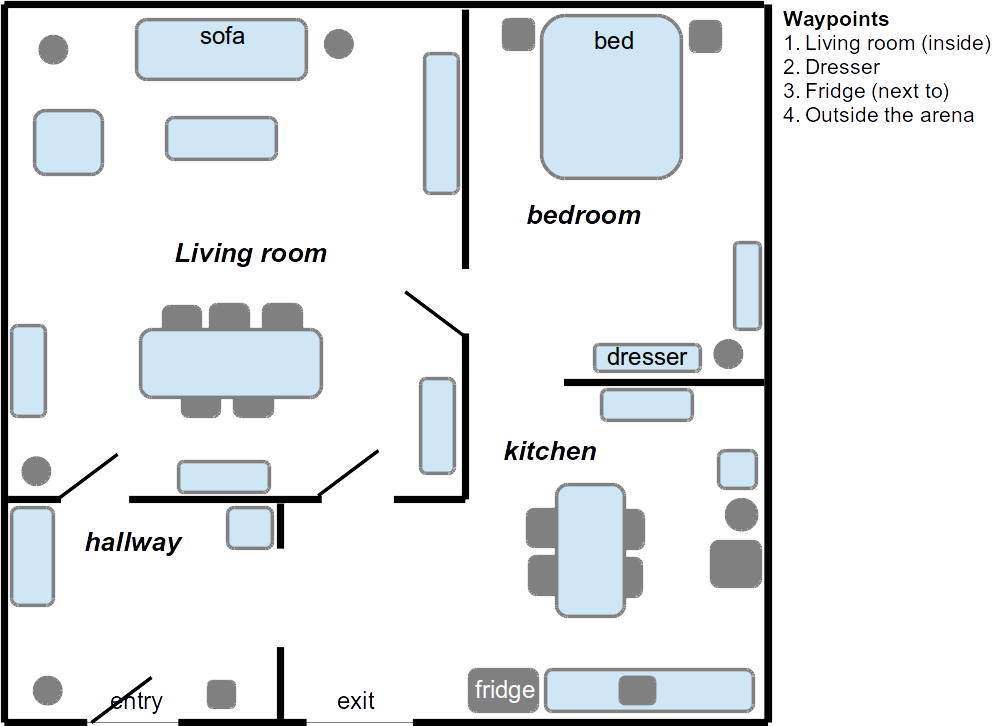
\includegraphics[width=0.5\columnwidth]{images/navigation.png}
	\caption{Navigation test: setup and execution example.}
	\label{fig:restaurant}
\end{figure}

\paragraph*{Remarks:}
\begin{enumerate}
	\item Depending on the layout of the arena, waypoint 1 and 2 may be swapped.
	\item Reaching a waypoint also includes the direction in which the robot should be looking when it reaches, which will be announced by the TC during the setup of the path.
	\item The distance between Waypoints 3 and 4 is about 10-20 meters.
\end{enumerate}

\subsection{Obstacles}
While navigating to waypoints 1, 2, and 3 the robot will find one of the following obstacles on its path:
\begin{itemize}
		\item \textbf{Small object:} Box sized object (between 5 and 15 cm per edge).  
		\item \textbf{3D Object:} A bar table, normal table, rolling chair: some object that is wider at its top than on its bottom, 
		  thus requiring more than just a laser scanner mounted near the ground to avoid obstacles.
		\item \textbf{Smart obstacle:} A person to whom the robot may speak to and kindly ask to move away. When interacting with people, the robot must look at the person and make clear is speaking with him/her.
	\end{itemize}

\subsection{Additional rules and remarks}
\begin{enumerate}
	\item \textbf{Waypoints:} Waypoints may be rooms, placement locations, furniture, beacons, landmarks, etc. The robot must clearly state when it has reached a waypoint or if it was not able to reach the waypoint.

	\item \textbf{Show must go on:} If a robot is unable to reach a waypoint, it must say it and proceed to the next one.

	\item \textbf{Closing internal doors:}  Theinternal door that will be shut will be the door on the route the robot has committed to. It will be shut right after the robot starts driving towards the door, but granting enough time to notice that the door is now closed.	

	\item \textbf{Moving objects:} If the robot finds on its way a \textit{static movable obstacle} (chair, cubes, toys, etc.) which is capable to move, it must announce is going to move an obstacle and then proceed to move the object apart with its manipulator, or by \textbf{gently} pushing it with its body.

	\item \textbf{Asking people to move away:} If the robot finds on its way a person blocking its path, it must announce it has found a person, \textit{gently} ask that person to move away and wait for the path to be clear. \textbf{Robots are not allowed to touch people}.

	\item \textbf{Following people:} 
	\begin{enumerate}
		\item \textbf{Instruction:} The robot interacts with the operator, \emph{not} the team. That is, the team is not allowed to instruct the operator.
		\item \textbf{Natural walking:} The operator has to walk \quotes{naturally}, i.e., move forward facing forward. 
		  The operator is not allowed to walk back, stand still, signal the robot or follow any re-calibration procedure.
		\item \textbf{Asking for passage:} The robot is allowed to (gently) ask people to step aside.
	\end{enumerate}
\end{enumerate}

\subsection{Data recording}
  Please record the following data (See \refsec{rule:datarecording}):
  \begin{itemize}
   \item Mapping data
   \item Plans
  \end{itemize}

\subsection{Referee instructions}

The referee needs to
\begin{itemize}
	\item Instruct the OC and volunteers on when and where locate objects.
	\item Instruct the OC and volunteers on when and which doors must be closed.
	\item Stop the robot immediately when it is about to collide.
\end{itemize}

\subsection{OC instructions}

\textbf{2 hours before the test}
\begin{itemize}
        \item Announce the entry and exit doors. 
	\item Announce the locations for waypoints 1, 2, and 3.
	\item Establish location for waypoint 4 and the path for the \textit{follow me} phase. 
\end{itemize}

\textbf{During the test}
\begin{itemize}
	\item Open and close the doors when instructed by the referee.
	\item Place the obstacles (or act as an obstacle) when instructed by the referee.
\end{itemize}

\newpage

\subsection{Score sheet}

The maximum time for this test is 5 minutes.

\begin{scorelist}

	\scoreheading{Waypoints}
	\scoreitem{10}{Reaching waypoint A}
	\scoreitem{10}{Reaching waypoint B}

	\scoreheading{Obstacles}
	\scoreitem{20}{Avoiding obstacle 1}
	\scoreitem{30}{Avoiding obstacle 2}
	\scoreitem{40}{Avoiding obstacle 3}
	\scoreitem{10}{Reporting unreachable waypoint due to an obstacle (will end the test)}

	\scoreheading{Doors}
	\scoreitem[2]{20}{Starting a new path after reaching a closed door}
	\scoreitem[2]{45}{Opening the door and continue instead of plan a new trajectory}

	\scoreheading{Optional tasks (up to 50 points)}
	\scoreitem{10}{Reaching waypoint}
	\scoreitem{40}{Reentering the arena after reach Waypoint 3}

	\setTotalScore{200}
\end{scorelist}


% Local Variables:
% TeX-master: "Rulebook"
% End:


% Local Variables:
% TeX-master: "Rulebook"
% End:


\subsection{Open/Demo Challenge}

The maximum time for this test is 5 minutes.

\begin{tabularx}{\textwidth}{X r c c c }

	\textbf{Action} & \textbf{Score} & \textbf{$1^{st}$ try} & \textbf{$2^{nd}$ try} & \textbf{$3^{rd}$ try} \\ \hline
	& & & & \\ 
	\textit{\textbf{Operator}} \\
	Approach or point at the operator & $30$ & \hrulefill & \hrulefill & \hrulefill \\
	Correctly state operator's gender & $30$ & \hrulefill & \hrulefill & \hrulefill \\
	Correctly state operator's pose & $30$ & \hrulefill & \hrulefill & \hrulefill \\
	& & & & \\ 
	\textit{\textbf{Crowd}} \\
	Correctly state crowd's size & $20$ & \hrulefill & \hrulefill & \hrulefill \\
	Correctly state crowd's number of men & $20$ & \hrulefill & \hrulefill & \hrulefill \\
	Correctly state crowd's number of women & $20$ & \hrulefill & \hrulefill & \hrulefill \\ \hline
	& & & & \\ 
	\textit{\textbf{Score per try}} & $150$ & \hrulefill & \hrulefill & \hrulefill \\ 
	& & & & \\ 
	\textbf{Total Score} & $150$ & & & \\ \cline{3-5}

\end{tabularx}\\


% Local Variables:
% TeX-master: "Rulebook"
% End:


\subsection{RoboZoo}

The maximum time for this test is 5 minutes.

\begin{scorelist}

	\scoreheading{Operator within the \textit{front range}}
	\scoreitem{10}{Correctly answered question 1}
	\scoreitem{10}{Correctly answered question 2}
	\scoreitem{10}{Correctly answered question 3}
	\scoreitem{10}{Correctly answered question 4}
	\scoreitem{10}{Correctly answered question 5}

	\scoreheading{Operator outside the \textit{front range}
	\footnotesize $2^{nd}$ attempt after asking operator to repeat the question}
	\scoreitem{20}{Correctly answered question 1 ($1^{st}$ attempt)}
	\scoreitem{10}{Correctly answered question 1 ($2^{nd}$ attempt)}
	\scoreitem{20}{Correctly answered question 2 ($1^{st}$ attempt)}
	\scoreitem{10}{Correctly answered question 2 ($2^{nd}$ attempt)}
	\scoreitem{20}{Correctly answered question 3 ($1^{st}$ attempt)}
	\scoreitem{10}{Correctly answered question 3 ($2^{nd}$ attempt)}
	\scoreitem{20}{Correctly answered question 4 ($1^{st}$ attempt)}
	\scoreitem{10}{Correctly answered question 4 ($2^{nd}$ attempt)}
	\scoreitem{20}{Correctly answered question 5 ($1^{st}$ attempt)}
	\scoreitem{10}{Correctly answered question 5 ($2^{nd}$ attempt)}

	\setTotalScore{150}
\end{scorelist}

% Local Variables:
% TeX-master: "Rulebook"
% End:



\chapter{Tests in Stage II}

\begin{itshape}
All ability and integration tests in Stage II grants 25 points and are performed only once. Some tests --like Wake-me-up Test-- have optional tasks that grant additional points when performed correctly, clean and fast. TC must be informed if a team is planning to perform any of the optional tasks. No additional time is given while performing optional tasks.
\end{itshape}

The maximum time for this test is 15 minutes.

\small\begin{scorelist}

	\scoreheading{Training phase}
	\scoreitem[3]{10}{Learning the location of a table (Professional Waiter)}
	\scoreitem[3]{5}{Learning the location of a table (Custom Waiter)}
	\scoreitem[3]{10}{Inferring the side on which a table is (Professional Waiter only)}
	
	\scoreheading{Ordering phase}
	\scoreitem{5}{Understanding which table to take an order from}
	\scoreitem{15}{Going to the designated table}
	\scoreitem{10}{Taking an order from the designated table}
	\scoreitem{20}{Noticing a waving/calling person from distance}
	\scoreitem{20}{Going to the table of the waving/calling person}
	\scoreitem{10}{Taking an order from the waving/calling person}
	\scoreitem{10}{Avoiding a person crossing the robots' path}

	\scoreheading{Delivering phase}
	\scoreitem[2]{5}{Reciting both the order and table number for both tables}
	\scoreitem{10}{Grasping the correct drink}
	\scoreitem{15}{Getting close to the correct table with the drink}
	\scoreitem{15}{Delivering the drink by placing it on the correct table}
	\scoreitem{15}{Picking up the plate}
	\scoreitem{15}{Getting close to the correct table with the plate}
	\scoreitem{20}{Delivering the plate by placing it on the correct table}

	\setTotalScore{250}
\end{scorelist}



% Local Variables:
% TeX-master: "Rulebook"
% End:


\newpage
\section{Robo-Nurse}

The robot is assisting an elderly person with getting her pills and responding to observed activities.

\subsection{Focus}

This test focuses mainly on Human-Robot Interaction and Activity Recognition.

\subsection{Task}
\begin{enumerate}
	\item \textbf{Start}: The robot is in a corner of the living room, the patient is sitting in the same room. 

	\item \textbf{Move to the patient}: The patient (lets call her Granny) calls for robot assistance using her voice or by waving arms.

	\item \textbf{Asking for pills}: Granny asks the robot for her pills which are in bottles located on a shelf nearby. 

	\item \textbf{Describe and choose pills}: On the shelf, there are multiple bottles with pills and the robot must asks Granny which bottle she needs.
	\begin{itemize}
		\item The robot must indicate what bottles are on the shelf by briefly describing each bottle.
		\textbf{the faster the robot starts describing (i.e.~finished recognizing) after arrival (standing still in front of the shelf) at the shelf, the better:} faster recognition gives more points. 
		\begin{itemize}
 			\item \quotes{The leftmost one}
  			\item \quotes{The \textit{color} bottle}
  			\item \quotes{The big/small bottle}
  			\item Any other description the robot understands and spoke out loud to Granny. E.g.~if a robot can do text recognition and read each label to Granny, she may reply with e.g.~\quotes{Aspirin}.
 		\end{itemize}
		\item \textbf{Describe unknown pills' bottles [Optional]:}. Team leader may request to use a set of pills' bottles which were not available beforehand for training (unknown to all robots). Additional points may be by Jury if the robot succeed in describing the unknown pills' bottles to Granny.
 	\end{itemize}

 	\item \textbf{Grasp \& handover pills}: The robot must grasp the indicated bottle of pills and hand them over to Granny. The handover to Granny must be \quotes{natural}, without a voice confirmation of when to let the pills go etc.~Granny will take the pills from the robot's hand and the robot must open its hand.

 	\item \textbf{Open pills bottle [Optional]:} After grasping a pills bottle, the robot may try to open it before delivering it to Granny.

 	\item \textbf{Give a single pill [Optional]:} If the robot succeeds opening the pills bottle, it may try to fetch a single pill from it to delivery to Granny.

 	\item \textbf{Activity Recognition}: One of the activities below happens and the robot must act accordingly:
 	\begin{itemize}
 		\item \textbf{Drop blanket}: Granny's stands up and sits down immediately. Her blanket falls over her lap on to the ground. The robot must \textbf{pick up the blanket} and hand it to Granny.

 		\item \textbf{Fall}: Granny stands up from her chair and falls. The robot must \textbf{hand Granny a phone}. The phone will be laying nearby, e.g.~on the coffee table in the living room. \\
		\textbf{[Optional]:} Robot may use Smart House option to do a phone call instead of delivering the phone to Granny.

 		\item \textbf{Walk and sit}: Granny walks to a table with her walking stick/cane. Robot must follow and take walking stick from Granny after she sits down an a chair nearby.
 	\end{itemize}
\end{enumerate}


\subsection{Additional rules and remarks}
\begin{enumerate}
	\item \textbf{Continue Rule:} The CONTINUE rule may be applied several times in the Conversation part of the test (Section \refsec{rule:asrcontinue}).

	\item \textbf{Make it fast:} Description of objects should be fast, as is reflected in the scoring.
	% \item The bottles of pills are not known beforehand and must be recognized and described on the spot by the robot. 
	
	\item \textbf{Opening pill bottles:} Provided pills' bottles will be chosen so they can be opened easily by twist, i.e.~no push and twist, no uncap, no seals nor any other complex opening method.

	\item \textbf{Optional tasks:} The test includes optional tasks (such as deliver the newspaper, placing the spoon, and doing bed) which are not required to be performed as part of the overall test but brings an additional scoring for solving it. Team leader must contact a TC member to request optional tasks to be available.

	\item \textbf{Smart-house:} The arena-house may have enabled official smart-house devices (Section \refsec{rule:smarthomedevices}), there are additional scoring for interacting with the house.
\end{enumerate}

\subsection{Referee instructions}

The referee needs to
\begin{itemize}
	\item Ask Team Leader whether they want known or unknown pills' bottles.
	\item Place the bottles on the shelf.
	\item Place the phone on announced position.
\end{itemize}

\subsection{OC instructions}

\textbf{2 hours before the test}
\begin{itemize}
	\item Announce the room where the patient is.
	\item Announce the room where the phone is.
\end{itemize}

\textbf{During the test}
\begin{itemize}
	\item Instruct Granny which pills she wants.
	\item Instruct Granny which of the 3 actions to perform.
\end{itemize}

\newpage 
\subsection{Score sheet}

The maximum time for this test is 10 minutes.

\begin{tabularx}{\textwidth}{ X r }
	\textbf{Action} & \textbf{Max.~score} \\ \hline
	\textbi{Attending request} \\
	Reach patient after being called & 2 \\
	Await command to get pills. & 1 \\
	\\
	\textbi{Describing pills} \\
	Real time description (given upon arrival) & 5 \\
	Description given within $t \leq 5$ seconds & 3 \\
	Description given within $5 < t \leq 15$ seconds & 2\\
	Description given within $15 < t \leq 30$ seconds & 1\\
	Wrong description given or $t > 30$ & 0\\
	\\
	\textbi{Picking pills} \\
	Choose the correct pills & 4 \\
	Grasp the correct pills & 2 \\
	Grasp wrong pills & 0.5 \\
	\\
	\textbi{Pills handover} \\
	Natural delivery (no instructions are given to operator) & 2 \\
	Assisted delivery (operator instructs robot for delivery) & 1 \\
	\\
	\textbi{Activity recognition} &  \\
	Granny trying to reach drop blanket & 5 \\
	Falling Granny & 5 \\
	Granny stands up and walk away\& sit & 5 \\
	\\
	\textbi{Response to activity} &  \\
	Pickup the blanket + give the blanket & 3+1 \\
	Grasp phone + give phone & 3+1 \\
	Take walking stick / cane & 4 \\ 
	\\
	\textbi{Bonuses (up to 18 points)} &  \\
	Using Smart House to call instead of grasping \& giving the phone & 1 \\
	(These are mutually exclusive) & \\
	Describe unknown pills' bottles & 3 \\
	Opening the pill bottle (with a screw cap) & 4 \\ 
	Picking a single pill from the bottle & 10 \\ \hline
	\textbf{Total score (excluding penalties and bonuses)} & 25
\end{tabularx}


\section{Wake me up test}

The robot's owner has overslept. Knowing the schedule of the owner and noticing it is getting late, the robot helps it's owner to wake up and start the day.

The robot has to help a human in a daily morning task. The task involves interact with a smart house, awake a dormant human, take an order, prepare the breakfast and deliver it to the human.

\subsection{Focus}

This test focuses on advanced object manipulation, human pose detection, object recognition and and manipulation; as well as object recognition.


\subsection{Task}

\begin{enumerate}

\item \textbf{Awakening the owner:} The robot enters the bedroom, approaches to the bed, and starts to awaken the owner (operator lying on the bed) for one minute by playing an alarm-like sound or using it's own voice. Within one minute starting from the first call, the owner will wake up in a natural way (sit on the bed and rub face; sit on bed, rise arms and yawn; stand up etc.), then the robot must announce it has successfully detected the awakening by greeting it's owner.
\begin{itemize}
\item \textbf{Turning-on bedroom's lights [Smart-house option]:} After entering to the bedroom, the robot can send a command to the house to turn on the bedroom lights.
\item \textbf{No annoying sounds:} Alarm-like sounds must be short and clean (no continuous music is allowed), and voice calls must be short and clear. A silence gap of 10 seconds between calls is advised.
\item \textbf{Show must go on:} One minute after the first call, the owner is awake, so the robot must proceed to the next point.
\end{itemize}

\item \textbf{Delivering the newspaper [Optional]:} After awakening it's owner, the robot approaches to her and delivers a newspaper into the owner's hand (the owner will face the robot after being awakened and extend her hand to it). Robot must release the newspaper only after the human has grasped it.

\item \textbf{Taking breakfast order:} The robot asks to it's owner for a breakfast of her preference. The order will include: one random fruit/snack, one kind of cereal, and one kind of milk (stating no milk means whole milk), but those can be given in any order. The robot may ask for a confirmation of the order up to three times. If the robot is not able to handle a tray (see below), it must state that breakfast will be delivered to the dining room. Examples of the order are:

\begin{itemize}
\item Froot-loops with banana and light milk.
\item Flakes with lactose-free milk and a peach.
\item Apple and choco-flakes (i.e. one apple, and choco-flakes with whole milk).
\end{itemize}

\item \textbf{Opening kitchen's door [Optional]:} The kitchen's door is closed. Upon arrival, robot has 1 minute to open the door. It may also give up and request for the door to be opened by a referee.

\item \textbf{Turning-on kitchen light [Smart-house option]:} After entering to the kitchen, the robot can send a command to the house to turn on the kitchen lights and the coffee brewer. Kitchen lights must be turned on every time the robot enters the kitchen.

\item \textbf{Serving the breakfast:} Once in the kitchen, the robot must locate the tray and place into it the requested fruit/snack, a box of the requested type of milk, and a bowl; then pour the requested type of cereal into the bowl. If the robot is not capable of handling a tray, it may serve the breakfast directly at the diner table. The placement order is not relevant.

\item \textbf{Placing the spoon [Optional]:} After placing the cereal bowl on the tray or dining room table, the robot may place a spoon close to it.
Delivering the tray: After placing objects into the tray, the robot must take the tray and deliver it to the human in the bedroom, leaving it on a table or directly to the owner's hands.

\item \textbf{Turning-off kitchen light [Smart-house option]:} After leaving to the kitchen, the robot can send a command to the house to turn off the kitchen lights. Kitchen lights must be turned off every time the robot leaves the kitchen.

\item \textbf{Doing the bed [Optional]:} After the breakfast has been delivered, the robot may proceed to do the owner's bed. Points are awarded based on a \quotes{Professional Mom} criteria.

\end{enumerate}

\subsection{Additional rules and remarks}

\begin{itemize}
\item \textbf{Smart-house:} The arena-house may have enabled official smart-house devices (Section \ref{rule:smarthomedevices}), there are additional scoring for interacting with the house.

\item \textbf{Optional tasks:} The test includes optional tasks (such as deliver the newspaper, placing the spoon, and doing bed) which are not required to be performed as part of the overall test but brings an additional scoring for solving it. Team leader must contact a TC member to request optional tasks to be available.

\item \textbf{Fruit or snack?:} If the robot is not able to properly handle fruits, it can be replaced by easier-to-manipulate objects from the official object list. Team leader must contact a TC member to request using snacks instead of fruits.

\item \textbf{Two robots:} This is a very challenging test and serving the breakfast is complex and time-consuming task. If a team has more than one robot, up to two robots may collaborate in the \quotes{serving the breakfast} and \quotes{delivering the tray} tasks. Team leader must contact a TC member to inform there will be two robots in the arena.

\item \textbf{Collaborative test:} The team leader may request help from a second team to perform the \quotes{serving the breakfast}, \quotes{delivering the tray} tasks, and \quotes{smart-house} optionals. All score achieved by both robots is given to the main team, but also the points scored by the helping-robot are given to the helping team as a bonus. This cooperation must be informed to the TC at least two hours before the competition.
\end{itemize}

\subsection{Referee instructions}

The referee needs to
\begin{itemize}
\item Give a wake-up signal to the operator within a minute starting from the robot started to call her
\item Generate and provide a random breakfast order for the operator
\item Type the breakfast order in a qualified typing device when required (Continue rule, Section \ref{rule:asrcontinue}).
\item Stop the robot immediately when tray is about to fall
\end{itemize}

\subsection{OC instructions}

\textbf{2 hours before the test}
\begin{itemize}
\item Announce the placement of the objects
\item Announce the placement of the tray

\end{itemize}
\textbf{During the test}
\begin{itemize}
\item Provide teams with the newspaper
\item Place tray and breakfast objects into the kitchen
\item Place spoon when needed
\end{itemize}

\subsection{Score sheet}
The maximum time for this test is 10 minutes.

\begin{tabularx}{\textwidth}{ X r }
	\textbf{Action} & \textbf{Score} \\ \hline
	\textbi{Awakening the human}  \\
	Detect the human awakening & 2.0 \\
	\\
	\textbi{Taking the order} \\
	Understanding whole order & 2.0 \\
	Understanding whole order on console (typed) & 0.5 \\
	Robot's own suggestion for breakfast & 0.0 \\
	\\
	\textbi{Serving breakfast} \\
	Placing the bowl & 2.0 \\
	Placing the milk bottle (½ score on wrong milk type) & 1.0 \\
	Placing the fruit/snack (½ score if using snack instead of fruit, ½ score on wrong object type) & 2.0 \\
	Pouring cereal into the bowl (½ score on wrong cereal type) & 3.0 \\
	Spilling cereal outside the bowl & -1.0 \\
	Spilling much cereal outside the bowl & -2.0 \\
	\\
	\textbi{Delivering breakfast} \\
	Grasping the tray (and successfully lifting it up to at least 5 cm for more than 10 second) & 3.0 \\
	Safely transporting the tray (no object inside flipped or fell during transport) & 1.0 \\
	Placing the tray (safely and the tray stands still for more than 10 second) & 2.0 \\
	Handing-over the tray to the operator's hands & 4.0 \\
	Complete the task with complete and correct order & 2.0 \\
	\\
	\textbi{Smart-House optionals} \\
	Turning on bedroom lights on enter & 1.0 \\
	Turning on kitchen lights and coffee brewer on enter & 1.0 \\
	Turning off kitchen lights on leave & 1.0 \\
	\\
	\textbi{Optional tasks (upt to 20 points)} \\
	Handing-over the newspaper & 2.0 \\
	Opening kitchen's door & 5.0 \\
	Placing the spoon & 3.0 \\
	Doing bed & 10.0 \\ \hline
	\textbf{Total score} (excluding optional tasks, penalties, and bonuses) & 25.0 \\
\end{tabularx}


\chapter{Finals}

\printabx
\printidx

\end{document}